\section{Introduction}
\label{sec:intro}

As students, we often hang out with our friends in pubs or in nightclubs. In those places, we usually have a few drinks, most of them containing alcohol. We are aware that this can be risky, and we also know that we should not exceed a certain amount, especially if we need to drive after the party. But the problem is that most of us do not know their limits, and do not realize how long it takes for their body to remove the alcohol. \\

To create a more alcohol-conscious society, there should be tools to inform the general crowd about the quantity of alcohol a person can ingest and the effects it will have on him or her. This is why we created Beerculator, an interactive tool which calculates the blood alcohol concentration based on the drinks that a person has had in a certain amount of time. It will also indicate how long the person has to wait before being sober again.\\

This is very important to provide such tools because it is proven that alcohol can have really bad effects on our behaviour. One of the most important of them is the increasing probability to cause accidents. The trend on {\sc figure}~\ref{fig:risks} should help you realize the consequences.

\vspace{2cm}

\begin{figure}[H]
	\centering
   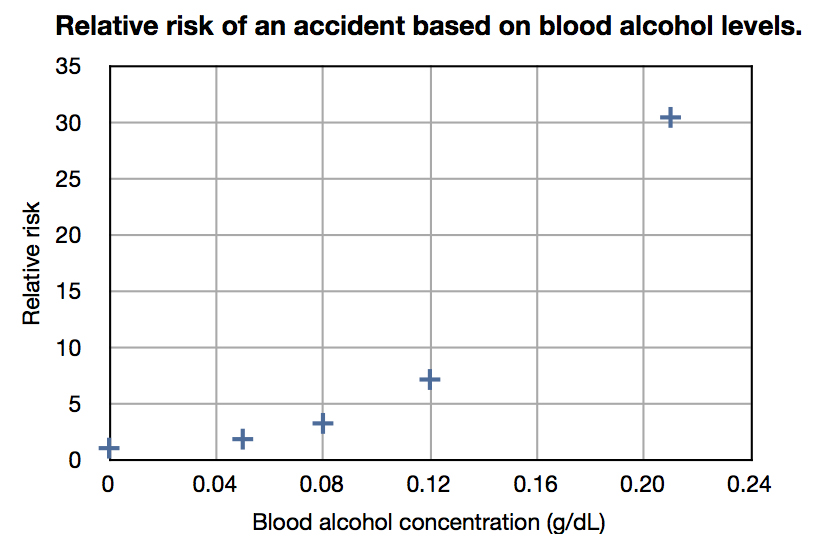
\includegraphics[scale=0.5]{./figures/risks.jpg}
   \caption{Relative risks of accidents based on the alcohol level}
   \label{fig:risks}
\end{figure}
